\section{Specifications}
\label{sec:Specifications}

\newcounter{rulei}[subsection]
\newcommand{\rcnii}{\stepcounter{rulei}\arabic{section}.\arabic{subsection}.\arabic{rulei}}
\renewcommand{\labelenumi}{\rcnii}

\subsection{Arena}
\begin{enumerate}
\item The match arena floor, overall, is an $8m \times 8m$ square (see \autoref{fig:arena-dim}).
 The tolerance of the two dimensions is $\pm0.25m$.
\item The width of the track is $1.5\pm0.1m$
\item The floor of the arena is made of white plastic coated hardboard.
 White Gaffer tape will be in place over the joints between hardboard sheets.
\item The outer arena walls are $600\pm30mm$ high and are made of the same material as the arena floor.
 The internal walls will be $200\pm30mm$ high, and also white.
\item A robot may not enter the area inside the internal wall.
\item No guarantee is offered of the colour of the area inside the internal wall (the section greyed out in \autoref{fig:arena-dim}).
 We can guarantee, however, that anything visible within the arena above $200mm$ and below $600mm$ will be either white or black (as those colours are not visible to the vision system).
\end{enumerate}

\subsection{The Ramp}
\label{sub:Ramp}
\begin {enumerate}
\item The ramp has the dimensions and shape shown in \autoref{fig:ramp-on-its-own}.
 This figure also shows the black, $60mm$ gaffer tape strip surrounding the arena.
\item The ramp has a footprint of $2.75m \times 1m$.
\item All track-facing vertical surfaces of the ramp are painted white.
\end {enumerate}

\begin{figure}
  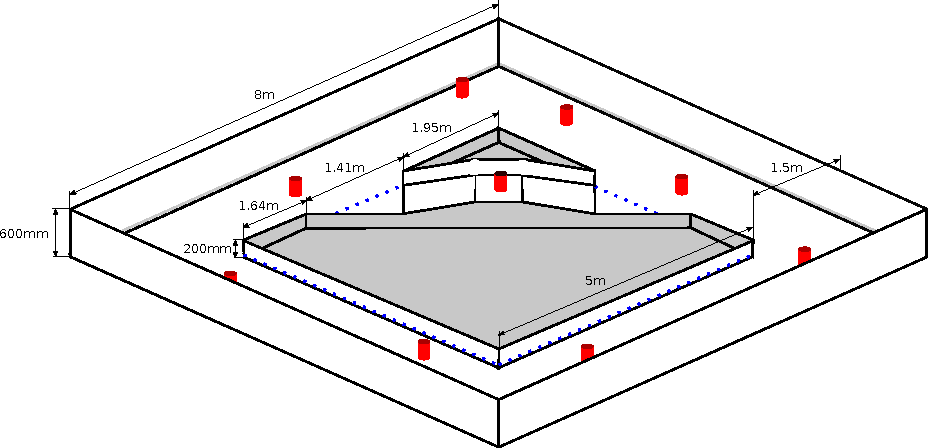
\includegraphics[keepaspectratio, clip, width=\textwidth]{./images/sr2011-arena.pdf}
  \caption{\label{fig:arena-dim}An overview of the arena --- including baked bean tin tokens --- with dimensions.}
\end{figure}

\begin{figure}
  \begin{center}
    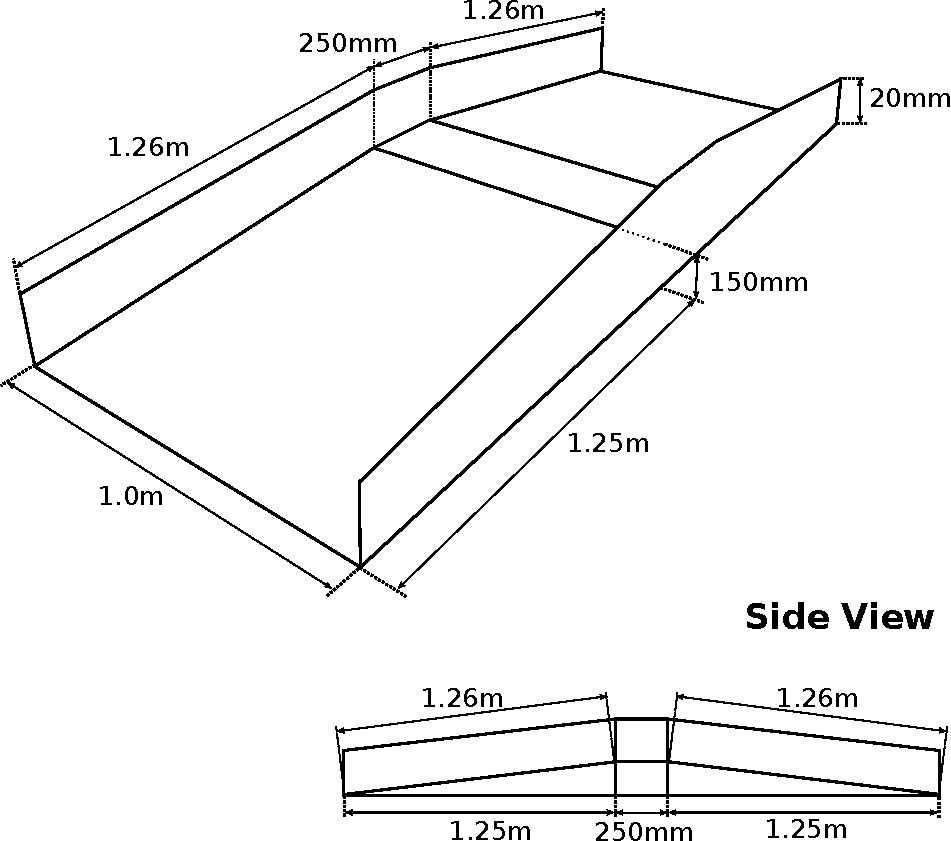
\includegraphics[keepaspectratio,width=\textwidth]{./images/ramp-2011.pdf}
  \end{center}
  \caption{\label{fig:ramp-on-its-own}The ramp that cuts one of the corners of the arena, as seen in \autoref{fig:arena-dim}.}
\end{figure}

\subsection{Tokens}
\label{sub:Tokens}
\begin {enumerate}
\item Tokens are baked-bean cans approximately $110mm$ high, with an approximate diameter of $75mm$.
 Each team's kit contains a small number of these.
\item Tokens have a mass of $400\pm30g$.
\item Tokens will be red.
\end {enumerate}

\subsection{Robot Flags}
\label{sub:Flags}

Robots \textbf{must} have a flag pole attached.
The top of the flag pole must be $1.1m$, measured from the floor.
A flag, of maximum size $200mm \times 200mm$ may be mounted $100mm$ from the top of the flag pole.
The flag \textbf{must not} sag below $800mm$ above the floor (this is to avoid interference with the vision system).
A $6mm$ diameter hole \textbf{must} be drilled at the top of the flag pole, no more than $10mm$ from the top of the flag pole.
The flag pole must be painted either green, white or black (this also avoids interference with the vision system).
The flagpole must be removable so that the robot can be placed within a box to check the size limit.

A diagram of the flagpole arrangement can be found in \autoref{fig:flag}.

\begin{figure}
 \begin{center}
  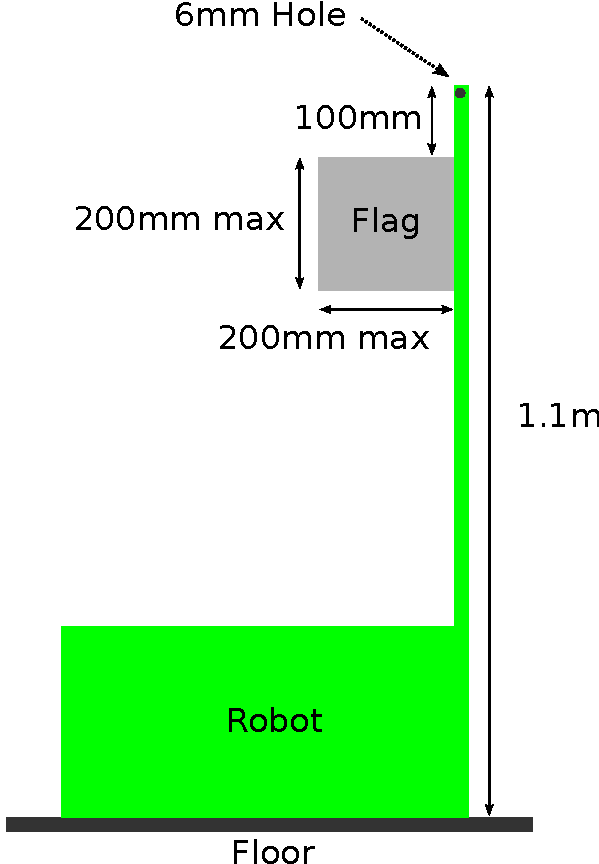
\includegraphics[keepaspectratio, scale =0.7]{./images/flag-2011.pdf}
  \caption{\label{fig:flag}Flagpole Dimensions}
 \end{center}
\end{figure}
\clearpage
